\documentclass{standalone}
\usepackage{tikz}

\begin{document}

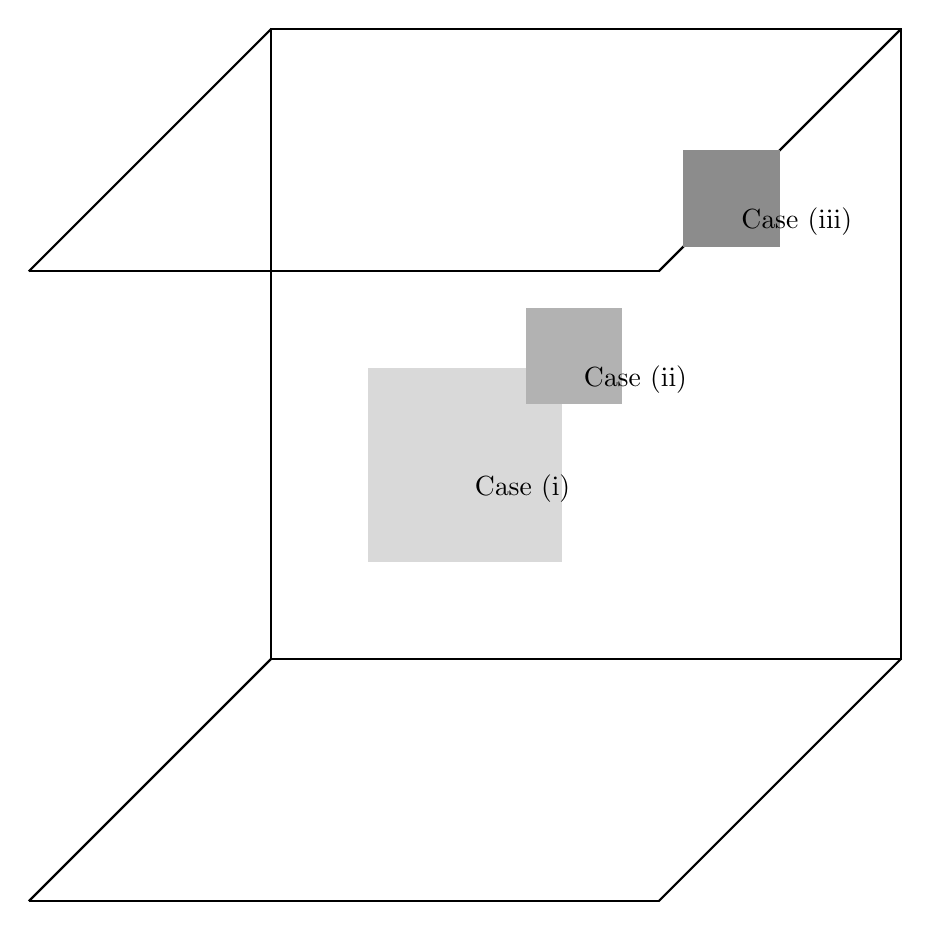
\begin{tikzpicture}[scale=2]

% Cube outline
\draw[thick] (0,0,0) -- (4,0,0) -- (4,4,0) -- (0,4,0) -- cycle;
\draw[thick] (0,0,0) -- (0,0,4);
\draw[thick] (4,0,0) -- (4,0,4);
\draw[thick] (0,4,0) -- (0,4,4);
\draw[thick] (4,4,0) -- (4,4,4);
\draw[thick] (0,0,4) -- (4,0,4);
\draw[thick] (0,4,4) -- (4,4,4);

% Case (i): Topology within the cube changes
\fill[gray!30] (1,1,1) rectangle (3,3,3);
\node at (2,2,2) [below right] {Case (i)}; 

% Case (ii): No topological change in B_w or connected cubes
\fill[gray!60] (2,2,1) rectangle (3,3,2);
\node at (2.5,2.5,1.5) [below right] {Case (ii)};

% Case (iii): Topological change outside B_w
\fill[gray!90] (3,3,1) rectangle (4,4,2);
\node at (3.5,3.5,1.5) [below right] {Case (iii)};

\end{tikzpicture}

\end{document}